\chapter{Τοπολογία Συστήματος}
\label{ch:System Topology}
Η δημιουργία μεταφέρσιμου (portable) λογισμικού, δηλαδή λογισμικού το οποίο μπορεί να χρησιμοποιηθεί σε συστήματα διαφορετικά μεταξύ τους, είναι δυνατή με τη χρήση αφαιρέσεων (abstractions) για το υποκείμενο σύστημα. Οι αφαιρέσεις αυτές αποκρύπτουν λεπτομέρειες της οργάνωσης του υλικού του εκάστοτε συστήματος, με την έννοια ότι από τη σκοπιά του προγραμματιστή δεν θα πρέπει να μας ενδιαφέρουν ζητήματα χαμηλού επιπέδου όπως για παράδειγμα η οργάνωση της μνήμης από φυσική άποψη (κοινόχρηστη ή κατανεμημένη) που αναφέραμε στην Υποενότητα \ref{ssec:Classification based on memory organization}, αλλά το τι εικόνα έχουμε για αυτή.

Η αφαιρετική όμως εικόνα που έχει ο προγραμματιστής για το σύστημα που καλείται να προγραμματίσει δεν του επιτρέπει να εκμεταλλευτεί στο μέγιστο τις δυνατότητές του και άρα να επιτύχει την καλύτερη δυνατή επίδοση. Για παράδειγμα, σε ένα σύστημα δύο κόμβων με κατανεμημένη φυσική οργάνωση μνήμης που όμως παρέχει κοινόχρηστο χώρο διευθύνσεων, ναι μεν ο ένας κόμβος μπορεί να προσβεί οποιαδήποτε θέση μνήμης στον άλλο κόμβο, παρόλα αυτά το κόστος της απομακρυσμένης πρόσβασης θα είναι πολύ μεγαλύτερο από αυτό της πρόσβασης στην τοπική μνήμη.

Στον προγραμματισμό παράλληλων συστημάτων που στόχος μας είναι η επίτευξη όσο το δυνατόν καλύτερων επιδόσεων, συχνά καταφεύγουμε στην εκμετάλλευση πληροφοριών που σχετίζονται με την τοπολογία. Για το λόγο αυτό γίνονται προσπάθειες δημιουργίας μεταφέρσιμου λογισμικού που όμως λαμβάνει υπόψην του την οργάνωση του υλικού σε χρόνο εκτέλεσης.

% Όπως αναφέραμε στην Υποενότητα \ref{ssec:Classification based on memory organization}, τα παράλληλα συστήματα μπορούν να ταξινομηθούν είτε βάσει της φυσικής οργάνωσης της μνήμης, είτε βάσει της εικόνας που έχει ο προγραμματιστής για αυτή, χωρίς όμως να υπάρχει απαραίτητα κάποια αντιστοίχιση μεταξύ των διαφορετικών τρόπων ταξινόμησης. Για παράδειγμα, ένα σύστημα με φυσικά κατανεμημένη μνήμη μπορεί να παρέχει κοινόχρηστο χώρο διευθύνσεων και άρα να προγραμματιστεί αντιστοίχως.


\section{Η εξέλιξη των βασικών στοιχείων ενός συστήματος}
Τα πιο σημαντικά στοιχεία που αποτελούν ένα υπολογιστικό σύστημα είναι αυτά που αφορούν τα υποσυστήματα επεξεργαστή και μνήμης.

Ένα απλό σειριακό σύστημα αποτελούνταν από έναν επεξεργαστή (ΚΜΕ - Κεντρική Μονάδα Επεξεργασίας, CPU - Central Processing Unit) ο οποίος περιείχε έναν επεξεργαστικό πυρήνα (ή απλώς πυρήνας, core) και επικοινωνούσε με την κύρια μνήμη μέσω ενός διαύλου. Με την εμφάνιση των πολυπύρηνων (multicore) οργανώσεων περισσότεροι του ενός πυρήνες ενσωματώθηκαν στον ίδιο επεξεργαστή, ενώ με την πάροδο του χρόνου προστέθηκε και ιεραρχία κρυφών μνημών.

Στα πλαίσια μιας άλλης αρχιτεκτονικής βελτίωσης, με μικρή αύξηση του μεγέθους του κυκλώματος, μπόρεσαν να ενσωματωθούν μέσα σε έναν πυρήνα 2 ή περισσότερα νήματα υλικού (H/W threads), ώστε να αξιοποιήθούν καλύτερα οι λειτουργικές μονάδες του επεξεργαστή, προσφέροντας με αυτό τον τρόπο τη δυνατότητα παράλληλης εκτέλεσης.

Τη σημερινή εποχή, μπορούμε να συναντήσουμε μεγάλα συστήματα που διαθέτουν πολλαπλούς επεξεργαστές, όπου κάθε επεξεργαστής είναι πολυπύρηνος, περιλαμβάνει ιεραρχία κρυφών μνημών και τοπική μνήμη, ενώ κάθε πυρήνας διαθέτει πολλαπλά H/W threads.

Στο Σχήμα \ref{fig:ideapad-topo} φαίνεται η οργάνωση ενός επεξεργαστή που διαθέτει 2 πυρήνες με 2 H/W threads και μία ιεραρχία κρυφών μνημών τριών επιπέδων (L1, L2, L3) στην οποία η κρυφή μνήμη του πρώτου επιπέδου διακρίνεται σε κρυφή μνήμη δεδομένων (L1d) και εντολών (L1i). Η οπτικοποίηση της τοπολογίας έγινε με το λογισμικό Portable Hardware Locality (hwloc) με το οποίο θα ασχοληθούμε περαιτέρω στην Υποενότητα Χ.

\begin{figure}[t]
	\centering
	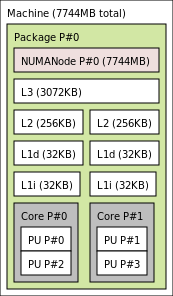
\includegraphics[width=0.25\textwidth]{Figures/ideapad-topo.png}
	\linebreak
	\caption{Η τοπολογία ενός Intel\textsuperscript{\textregistered} Core\textsuperscript{\texttrademark} i3-7100U.}
	\label{fig:ideapad-topo}
\end{figure}


\section{Συστήματα NUMA}
\label{sec:NUMA Systems}
Στην Υποενότητα \ref{ssec:Classification based on memory organization} περιγράφηκε η οργάνωση των συστημάτων ανομοιόμορφης προσπέλασης μνήμης (NUMA), τα οποία αποτελούν αρχιτεκτονική εξέλιξη των Συμμετρικών Πολυεπεξεργαστών (SMPs) που επιτρέπει την κατασκευή μεγαλύτερων παράλληλων συστημάτων.

Η πιο συχνή υλοποίηση των συστημάτων NUMA είναι ως ένα σύνολο κόμβων τύπου SMP που διαθέτουν ιεραρχία κρυφών μνημών συνδεδεμένους μεταξύ τους με ένα δίκτυο διασύνδεσης \cite{dobson2003linux}. Το δίκτυο διασύνδεσης μπορεί να είναι δακτύλιος (ring), διακοπτικό δίκτυο τύπου crossbar, από σημείο σε σημείο (point-to-point) ή πλέγμα (mesh).

Η εξασφάλιση της συνοχής των κρυφών μνημών συνήθως επιτυγχάνεται με τη χρήση ενός πρωτοκόλλου εντός του κόμβου και ενός δεύτερου πρωτοκόλλου μεταξύ των κόμβων. Όπως αναφέρθηκε νωρίτερα, ένας κόμβος SMP βασίζεται σε δίαυλο, ενώ η επικοινωνία μεταξύ των κόμβων γίνεται με πιο πολύπλοκα δίκτυα διασύνδεσης. Για το λόγο αυτό, το πρωτόκολλο συνοχής εντός του κόμβου είναι τύπου παρακολούθησης (snooping protocol), ενώ αυτό μεταξύ των κόμβων βασίζεται σε καταλόγους (directory-based protocol). Φυσικά, σε διαφορετικές οργανώσεις συστημάτων NUMA μπορούμε να συναντήσουμε και άλλες στρατηγικές επίτευξης συνοχής, όπως αυτή της μη αποθήκευσης κοινόχρηστων δεδομένων στις κρυφές μνήμες.

Όπως γίνεται γρήγορα αντιληπτό, ο προγραμματισμός αυτών των συστημάτων συνήθως απαιτεί να εστιάσουμε στην τοπικότητα, δηλαδή τη χρήση πόρων που βρίσκονται στη μικρότερη δυνατή απόσταση και την μείωση της επικοινωνίας μεταξύ των κόμβων \cite{bligh2004linux}. Για την επίτευξη της τοπικότητας και άρα τη συγγραφή πιο αποδοτικών προγραμμάτων, η εκμετάλλευση πληροφορίας που σχετίζεται με την τοπολογία είναι απαραίτητη.

% Ήδη από την έκδοση 2.5 του Linux Kernel προστέθηκε η βασική υποδομή για υποστήριξη συστημάτων NUMA, που περιλαμβάνει μεταξύ άλλων αναγνώριση της τοπολογίας, δέσμευση μνήμης και χρονοδρομολόγηση διεργασιών \cite{dobson2003linux}.

Στο Σχήμα \ref{fig:parade-topo} φαίνεται η οργάνωση του \texttt{parade}, ενός NUMA συστήματος με τέσσερις κόμβους τύπου SMP που διαθέτει η Ομάδα Παράλληλης Επεξεργασίας του Πανεπιστημίου Ιωαννίνων.

\begin{figure}[t]
	\centering
	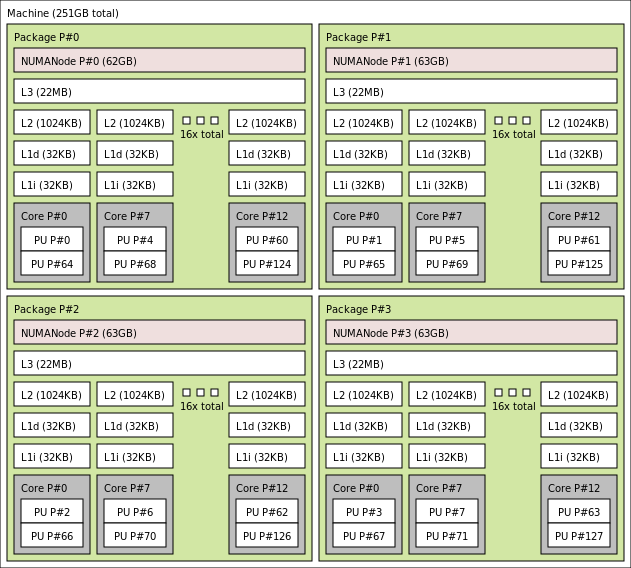
\includegraphics[width=0.8\textwidth]{Figures/parade-topo.png}
	\linebreak
	\caption{Η τοπολογία ενός Dell PowerEdge R840 με 4 Intel\textsuperscript{\textregistered} Xeon\textsuperscript{\textregistered} Gold 6130.}
	\label{fig:parade-topo}
\end{figure}

\section{Βοηθητικά Εργαλεία}
\label{sec:Utility Tools}
Η διπλωματική εργασία περιέχει $\nu$ κεφάλαια.


\section{Χρήση τοπολογίας στο OpenMP}
\label{sec:Topology in OpenMP}
Η διπλωματική εργασία περιέχει $\nu$ κεφάλαια.
